\chapter{Methodology}
\label{cp:Methodology}



\section{Maximum variance of sliding-window}
\label{sec:maxvar}
We assume that the pixels on the surface of the phone's cover are homogeneous. Therefore, an idea of using the variance of pixel values to extract features representing the state of the surface is proposed.



The control charts are used spatially by moving a mask (or window) across the image and then calculating and plotting a statistic each time the mask is moved. The size of the mask depends on the expected size of the defects to be detected, with smaller defective regions requiring smaller mask sizes~\cite{megahed2011review}. Inspired by this view, we move a ten by ten window (The size of the window is obtained by measuring the smallest size of defective region) across the image and calculate the variance of the pixel value each time the window is moved. The value with the largest variance among all windows in this image is taken as the desired statistic (maximum-variance) describing this image.


\section{Sliding-windows based $\bar{X}$ control chart}
In this section we combine Shewhart $\bar{X}$ control chart with sliding-window approach to perform statistical monitoring of image data. 
In Section~\ref{sec:maxvar} a statistic "maximum-variance" is retrieved from a image. Thus in Phase I $n$ standard sample images are used as Phase I data to retrieve the mean value ($\overline{m}$)

\begin{equation}
\overline{m}=\frac{1}{n} \sum_{i=1}^{n} m_{i}\,,
\label{equ:m_mean}
\end{equation}

and sample standard deviation ($ \sigma_{s} $) according to Equation\eqref{equ:sigma}-\eqref{equ:sigma_s} 

\begin{equation}
    \sigma_{s}=\frac{s}{c_{4}} \sqrt{1-c_{4}^{2}}\,,
    \label{equ:standarg_deviation}
\end{equation}

of the samples' statistic (maximum variance). In Phase II, by selecting $k = 3$, Equation~\ref{equ:UCL} become 

\begin{equation}
    U C L=\mu_{m}+3 \sigma_{s}\,,
    \label{equ:UCL_real}
\end{equation}

and LCL according to Equation~\ref{equ:LCL} is then

\begin{equation}
    U C L=\mu_{m}-3 \sigma_{s}\,.
    \label{equ:LCL_real}
\end{equation}
They will form a qualified range for the maximum-variance of the sample.
we will monitor whether the maximum-variance of the incoming sample is within this range. If it is the case, this sample will be considered qualified. Otherwise, it is unqualified.

\section{Haar Wavelet decomposition}
\label{sec:dwt}
As mentioned in the Section~\ref{cp:Background}: The DWT [Figure~\ref{fig:dwt}] analyzes the signal at different frequency bands with different resolutions by decomposing the signal into a coarse approximation and detail information, which is associated with low-pass and high-pass filters, respectively. In our case we employ the Haar Wavelet Transform (HWT) as the wavelet basic function to perform image decomposition so that an original image is decomposed into four coefficient matrices: one low-pass filtering coefficient matrix (approximation coefficient matrix $\mathbf{A}$) and three high-pass filtering coefficient matrices (detail coefficient matrices, containing the horizontal ($\mathbf{H}$), vertical ($\mathbf{V}$), and diagonal ($\mathbf{D}$) detail coefficient matrix) at each level. HWT is one of the simplest yet powerful transformations. It is first proposed by Hungarian mathematician Alfréd Haar (1910)~\nocite{haar1910theorie}. The base transformation of HWT in the multiple level scaling space is

\begin{equation}
\begin{aligned}
\centering&I_{i}^{j}=\frac{1}{2}\left(I_{2 i}^{j+1}+I_{2 i+1}^{j+1}\right)\,, \\
\centering&D_{i}^{j}=\frac{1}{2}\left(I_{2 i}^{j+1}-I_{2 i+1}^{j+1}\right)\,,
\end{aligned}
\end{equation}

in which $j$ is the level of scaling space, $I_{i}$ is $i-th$ value of discrete signal I. $I_{i}^{j}$ is the average of $j+1$ level's values of two contiguous pixels, which correspond to coarse approximation of level $j$, while $D_{i}^{j}$ is the difference of $j+1$ level's pixels value of two contiguous pixels corresponding to detail information of level $j$. 

\begin{figure}[h]
\centering
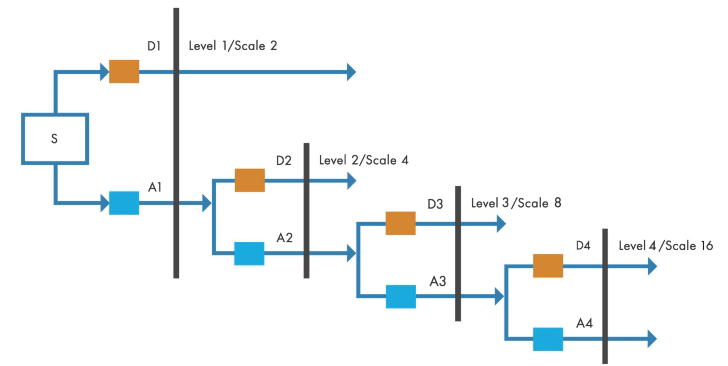
\includegraphics[width=1\textwidth]{images/dwt.png}
\caption{A general structure of DWT. The orange cube represent high-pass filter, the blue cube represent low-pass filter.}
\label{fig:dwt}
\end{figure}


%~\cite{polikarTHE WAVELET TUTORIALusing}
In this study the format of signal is the RGB-image of ($M \times N \times 3$). We use haar transform to decompose the image to finest scale so that high-level statistics are retrieved to represent the characteristic of image. This procedure is also known as dimensionality reduction. 

Since the analyzed images are in the form of 2-D, we need to perform the 2-D Haar wavelet transform by applying 1-D wavelet transform first on rows and then on columns. Based on the transfer concept of the one dimensional space, the Haar wavelet transform can process a two-dimensional image of ($M \times N$) pixels each level in the following way:

\begin{equation}
\begin{aligned}
\centering&\mathbf L=\frac{1}{2} * \left(\mathbf I\left(:, 1:2:N\right)+\mathbf I\left(:, 2:2:N\right)\right)\,, \\
\centering&\mathbf H=\mathbf I\left(:, 2:2:N\right)-\mathbf I\left(:, 1:2:N\right)\right)\,,
\label{equ:haar_wavelet1}
\end{aligned}    
\end{equation}

where $\mathbf I$ is the $M \times N$ matrix represent 2-D image, the bold letter with parentheses at $\mathbf I\left( a:b, c:d \right)$ represent matrix slicing and the range of slicing is from row $a$ to $b$, column $c$ to $d$. $\mathbf I\left(:, 1:2:N\right)$ extract all the odd column elements of matrix $\mathbf I$, $\mathbf I\left(:, 2:2:N\right)$ extract all the even column elements of matrix $\mathbf I$. The dimension of $\mathbf L$ and $\mathbf H$ is now $M \times \frac{N}{2}$. Symbols $+$, $-$ and $*$ here are matrix addition operation, which add the corresponding elements in two matrices together, matrix subtraction operation, which subtract corresponding elements in two matrices, and matrix scalar multiplication, in which the scalar is a constant and multiply every elements in the matrix, respectively. The prerequisites of matrix $\pm$ operation are that the order of the matrices must be the same, while by scalar multiplication the matrix can be any order.

\begin{equation}
\begin{aligned}
\centering&\mathbf A=\mathbf L(2:2:M,:)+\mathbf L(1:2:M,:)\,,\\
\centering&\mathbf V=\mathbf L(2:2:M,:)-\mathbf L(1:2:M,:)\,, \\
\centering&\mathbf H=\frac{1}{2} * \left(\mathbf H(2:2:M,:)+\mathbf H(1:2:M,:)\right)\,,\\
\centering&\mathbf D=\frac{1}{2} * \left(\mathbf H(2:2:M,:)-\mathbf H(1:2:M,:)\right)\,,
\label{equ:haar_wavelet2}
\end{aligned}    
\end{equation}

$\mathbf L(1:2:N,:)$ and $\mathbf H( 1:2:N,:)$ extract all the odd row elements of matrix $\mathbf L$ and $\mathbf H$ respectively. After the matrices operation, The dimention of the coefficient matrix $\mathbf A$, $\mathbf V$, $\mathbf H$, and $\mathbf D$ is then $\frac{M}{2} \times \frac{N}{2}$. Coefficient matrix $\mathbf A$ can be considered as a smooth subimage and represents the coarse approximation of the image $\mathbf I$, while coefficient matrix $\mathbf H$, $\mathbf V$, and $\mathbf D$ correspond to detail subimages and represent the horizontal, vertical and diagonal directions of the image $\mathbf I$ at corresponding level, respectively. The number of coefficients for matrices $\mathbf A$ $\mathbf H$ $\mathbf V$, and $\mathbf D$ is halved each time the level increase.


%The Haart2 transform is obtained down to level
The lowest level ($L_l$) that can be obtained by the HWT is

\begin{equation}
L_l= \log_2(min(r,c)) \label{equa:log1}
\end{equation}

%\[\log_2(min(row's dimension,column's dimension))\] \label{equa:log1}
If the row or column dimension of data is even, but not a power of two, the lowest level ($L_l$) that can be obtained by the HWT transformation is

\begin{equation}
L_l = \lfloor \log_2\left(\frac{min(r,c)}{2}\right) \rfloor 
\label{equa:log2}
\end{equation}

where $r$, $c$ is the row and column dimension of image, respectively, and the symbol $\lfloor E \rfloor$ rounds element $E$ to the nearest number.
%\[\lfloor \log_2(\frac{min(row's dimension,column's dimension)}{2}) \rfloor\] \label{equa:log2}

%In our case, we have sample data of size 100 * 100. The largest level of Haart2 transform is then five by using Equation \ref{equa:log2}.By using wavelet decomposition







\section{Wavelet decomposition based Hotteling $T^{2}$ control chart}
In order to monitor the surface quality of the mobile phone's cover, feature statistics are needed to characterize the quality of the cover.
Lin (2007) ~\nocite{lin2007automated} used wavelets and multivariate statistical approaches, including the Hotelling $T2$ control charts, to detect ripple and other types of defects in electronic components, particularly surface barrier layer (SBL) chips of ceramic capacitors. 
The specific approach first divides a grayscale image of $(256 \times 256)$ pixels into a set of equal-size sub-images of $(4 \times 4)$ pixels. The multivariate statistic (e.g. $T^{2}$) integrates the multiple wavelet characteristics ($h$, $d$, $v$) into a statistic value for each sub-image. This statistic value can be regarded as a distance value of the sub-image. The larger the statistic value, the larger the difference between the region and the normal area, the more that region can be judged as a defect region. Finally, a $T^{2}$ spatial distribution map of the image combined with $T^{2}$ statistic of sub-images is generated. The localization of the defect of the product can be achieved by finding the high value of the $T^{2}$ spatial distribution map. 


Since our goal is to monitor whether an RGB image with three frames: Red (R), Green (G), and Blue (B) frame is qualified or not, the location of the defect is not our concern. We apply Haar wavelet transform on each image. The coefficients of the final level ($L_l$) have $L$ times filtered by the high pass filter, which means the amplitude of coefficients contains the information of the high-frequency signal in the original image. The higher the coefficients, the more likely the signal will be abrupt. The abrupt in the signal then correspond to the defects in the monitored products.
% maybe I should try to get 9 elements to represent an image, that is more reasonable


According to Equation\eqref{equ:haar_wavelet1}-\eqref{equa:log2}, an image can be decomposed into horizontal ($\mathbf{H}$), vertical ($\mathbf{V}$), diagonal ($\mathbf{D}$), and approximation ($\mathbf{A}$) coefficient matrix ($S \times S$) at final level ($L_l$), each coefficient matrix have $S^2$ coefficients,an image sample can have $4 \times S^2$ coefficients.

Montgomery (2020) present tables indicating the recommended number of quality characteristics $p$ = 2, 3, 4, 5, 10, and 20. Here we use $p$ = 3, namely 3 maximum coefficient retrieved from $\mathbf{H}$, $\mathbf{V}$, and $\mathbf{D}$ coefficient matrices, since the coefficients of the each coefficient matrix reflect the surface defects of various shapes by experiment~\ref{subsec:hvd_experiment}. We absolute all coefficients of $\mathbf{H}$, $\mathbf{V}$, and $\mathbf{D}$ matrix

\begin{equation}
\begin{aligned}
&{[\mathbf{H}]=\text { absolute }[\mathbf{H}]} \\
&{[\mathbf{V}]=\text { absolute }[\mathbf{V}]} \\
&{[\mathbf{D}]=\text { absolute }[\mathbf{D}]}
\end{aligned}
\label{equ:absD}
\end{equation}



which turn negative coefficients into positive coefficients without changing the value itself.


After that, we take the maximal coefficient of $\mathbf{H}$, $\mathbf{V}$, and $\mathbf{D}$ matrix and consider them the desired statistical characteristics ($d1$,$d2$,$d3$) of the corresponding coefficient matrix. 

\begin{equation}
\begin{aligned}
&{[d1]=\text { max }[\mathbf{H}]} \\
&{[d2]=\text { max }[\mathbf{V}]} \\
&{[d3]=\text { max }[\mathbf{D}]}
\end{aligned}
\label{equ:maxD}
\end{equation}

Further, three coefficients retrieved from three frames compose the multiple wavelet characteristic vector $\mathbf{x}$. 

\begin{equation}
\mathbf{x}=\text { [d1,d2,d3] }
\end{equation}

These procedures are illustrated in Figure ~\ref{fig:dwt_procedure}. Finally, the Hotelling $T^{2}$ statistic

\begin{figure}[h]
\centering
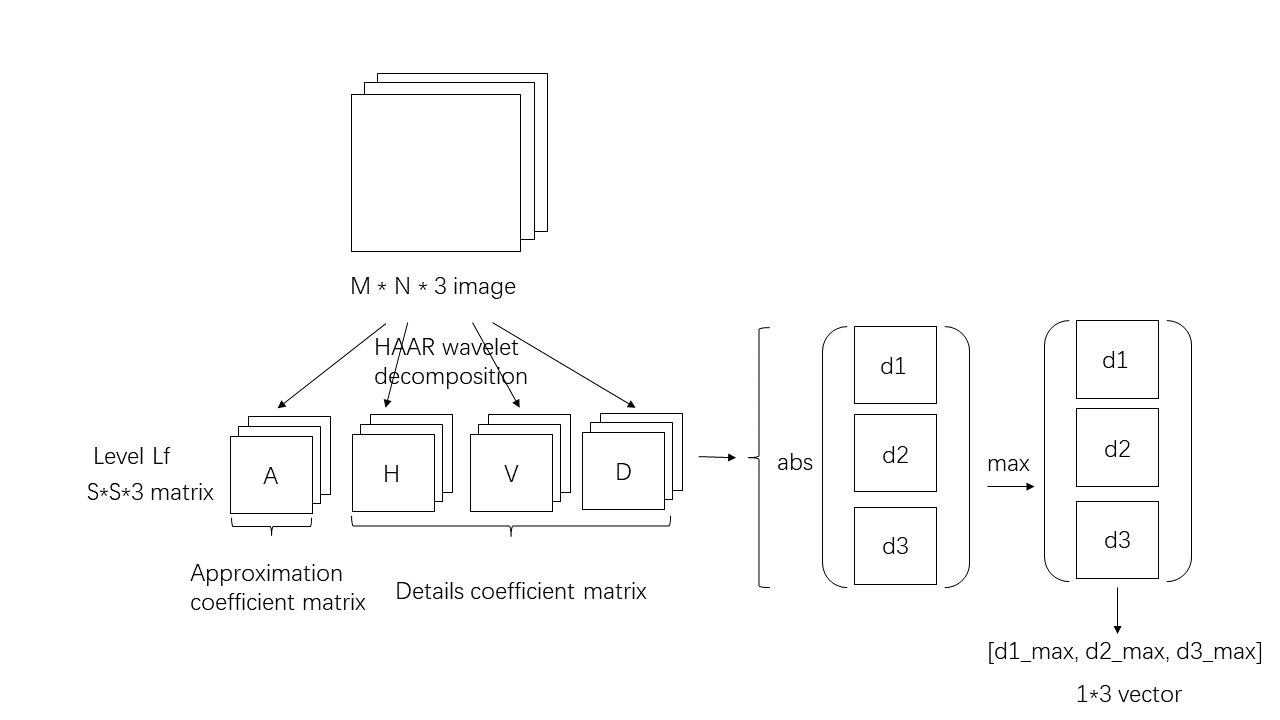
\includegraphics[width=1\textwidth]{images/wavelet_process.png}
\caption{Decomposition of RGB image into $1\times3$ wavelet characteristic vector}
\label{fig:dwt_procedure}
\end{figure}


\begin{equation}
\centering T^{2}=(\mathbf{x}-\overline{\mathbf{x}})^{\prime} \mathbf{S}^{-1}(\mathbf{x}-\overline{\mathbf{x}}) \label{equa:T2}
\end{equation}

in which $\overline{\mathbf{x}}$ and $\mathbf{S}$ be the sample mean vector and
covariance matrix, respectively, of these observations,
integrates the multiple wavelet characteristics $\mathbf{x}$ into a statistic value $T^{2}$ for each sample image.
If this statistic value is larger than UCL (Equation~\ref{equ:UCL_T2}), then we are $(1 - \alpha)$ confident that this sample is out of control. Vice versa, we are $(1- \alpha)$ confident that this sample is in control.


The output of the Phase I (the sample mean vector $\overline{\mathbf{x}}$ and covariance matrix $\mathbf{S}$ of standard images as well as UCL) is used as the input of Phase II. The images in Phase II are first decomposed by Haar wavelet transform into $3 \times 1$ characteristic vector $\mathbf{x}$. Then by using Equation~\ref{equa:T2} we can calculate the Hotelling $T^{2}$ statistic of this sample and compare it with UCL to judge if the sample is in control.



%Multivariate Control Chart can be utilized to simultaneous monitor more than one quality characteristic.





